\documentclass{standalone}
\usepackage{tikz}
\usetikzlibrary{patterns, positioning}
\usepackage[sfdefault]{ClearSans} %% option 'sfdefault' activates Clear Sans as the default text font
\usepackage[T1]{fontenc}

\begin{document}
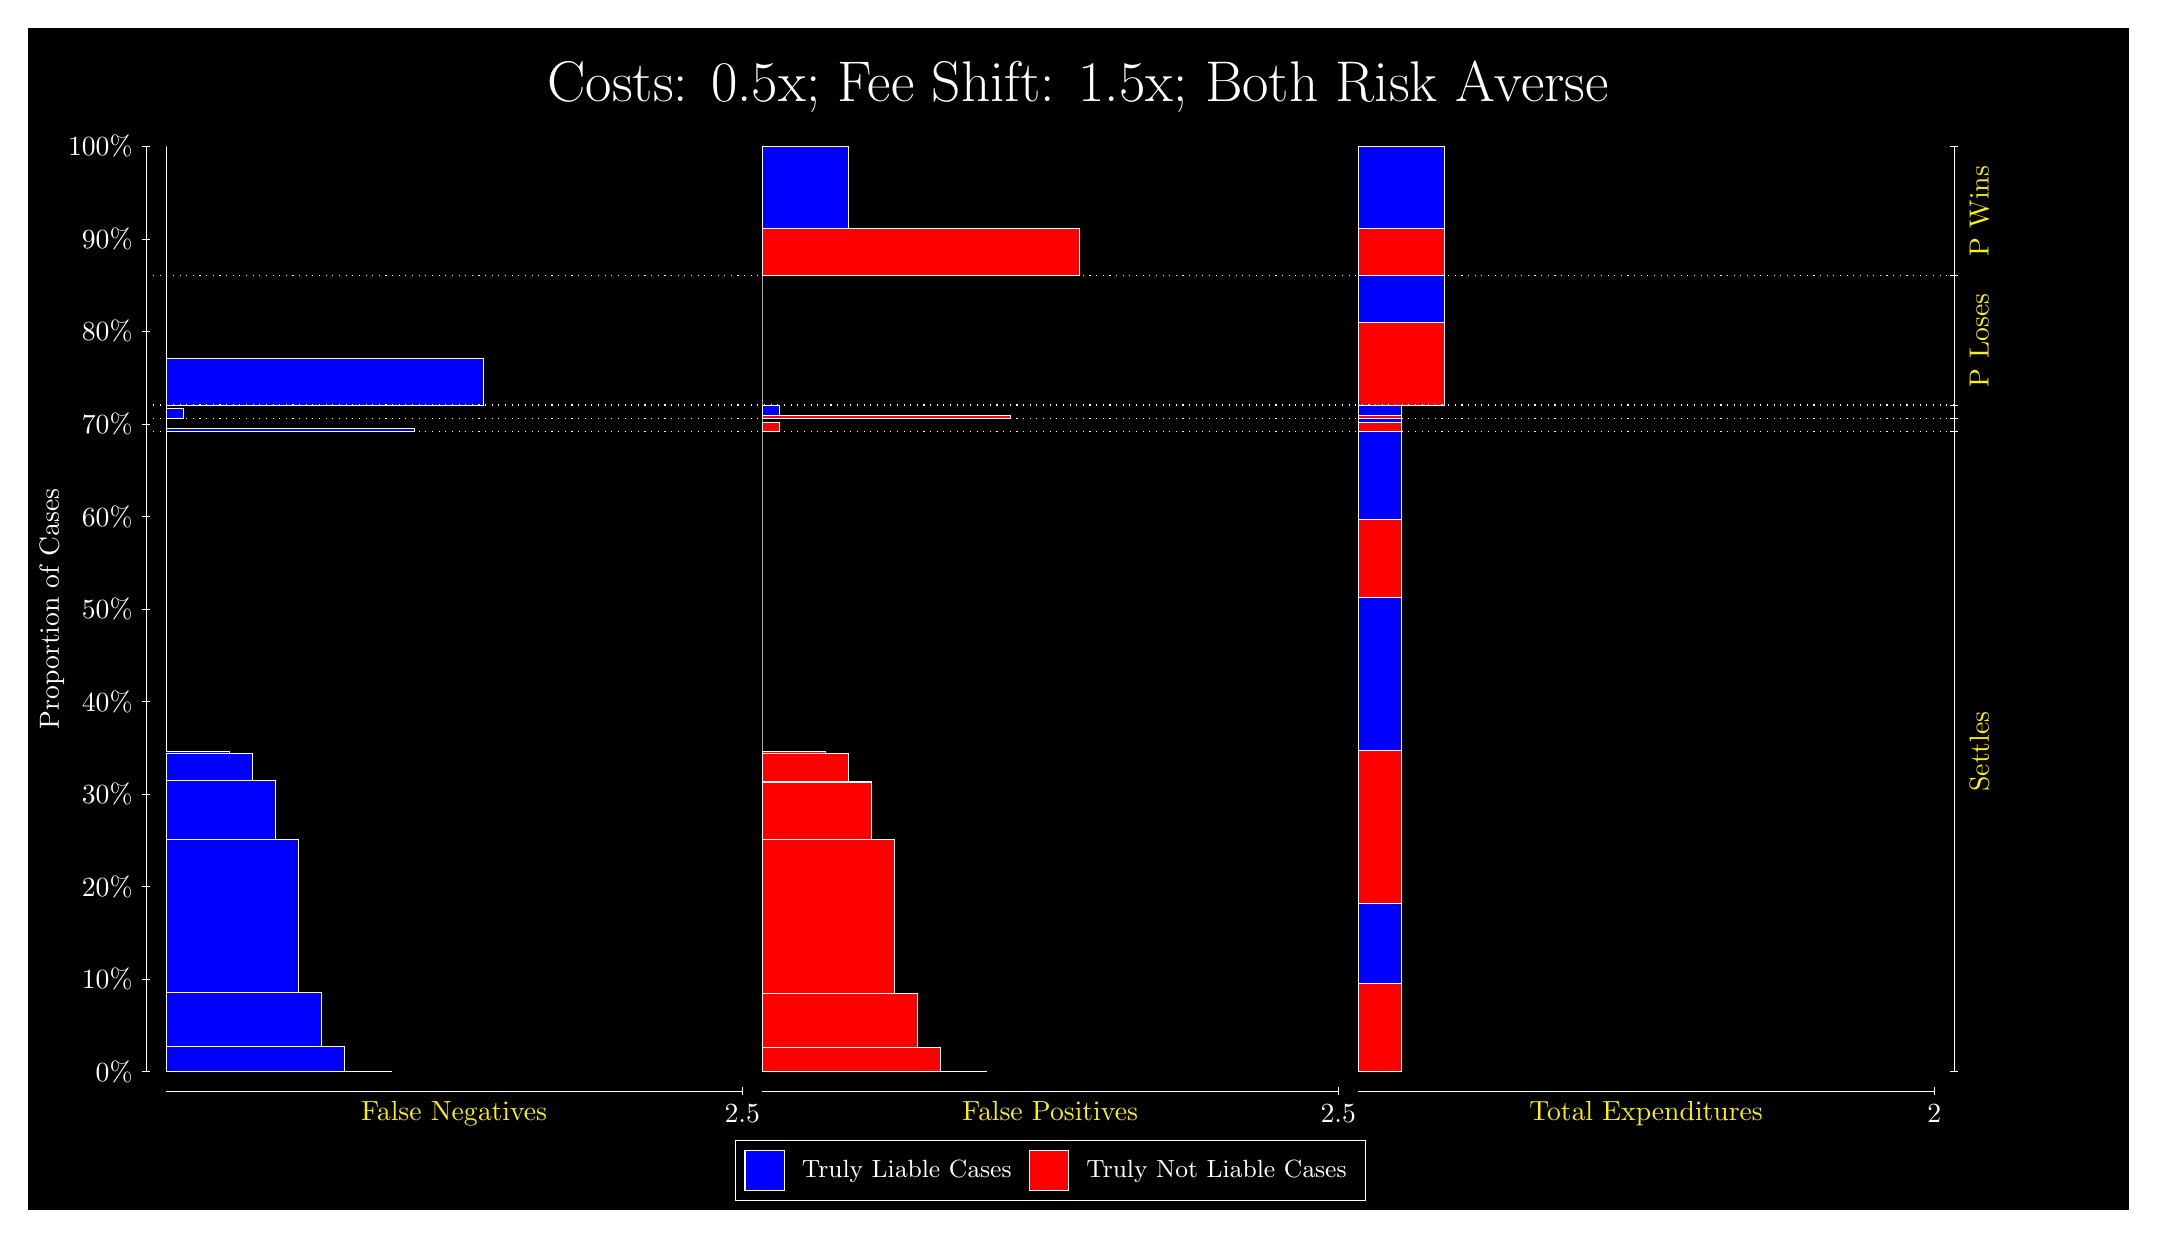
\begin{tikzpicture}
\draw[fill=black] (0,0) rectangle (26.667,15);
\draw[text=white] (0,13.5) rectangle (26.667,15) node[midway] {\huge Costs: 0.5x; Fee Shift: 1.5x; Both Risk Averse};
\draw[white, very thin] (1.5,1.75) -- (1.5,13.5);
\node[rotate=90, text=white, anchor=center] at (0.3, 7.625) {Proportion of Cases};
\draw[white, very thin] (1.45,1.75) -- (1.55,1.75);
\node[text=white, anchor=east] at (1.45, 1.75) {0\%};
\draw[white, very thin] (1.45,2.925) -- (1.55,2.925);
\node[text=white, anchor=east] at (1.45, 2.925) {10\%};
\draw[white, very thin] (1.45,4.1) -- (1.55,4.1);
\node[text=white, anchor=east] at (1.45, 4.1) {20\%};
\draw[white, very thin] (1.45,5.275) -- (1.55,5.275);
\node[text=white, anchor=east] at (1.45, 5.275) {30\%};
\draw[white, very thin] (1.45,6.45) -- (1.55,6.45);
\node[text=white, anchor=east] at (1.45, 6.45) {40\%};
\draw[white, very thin] (1.45,7.625) -- (1.55,7.625);
\node[text=white, anchor=east] at (1.45, 7.625) {50\%};
\draw[white, very thin] (1.45,8.8) -- (1.55,8.8);
\node[text=white, anchor=east] at (1.45, 8.8) {60\%};
\draw[white, very thin] (1.45,9.975) -- (1.55,9.975);
\node[text=white, anchor=east] at (1.45, 9.975) {70\%};
\draw[white, very thin] (1.45,11.15) -- (1.55,11.15);
\node[text=white, anchor=east] at (1.45, 11.15) {80\%};
\draw[white, very thin] (1.45,12.325) -- (1.55,12.325);
\node[text=white, anchor=east] at (1.45, 12.325) {90\%};
\draw[white, very thin] (1.45,13.5) -- (1.55,13.5);
\node[text=white, anchor=east] at (1.45, 13.5) {100\%};

\draw[white, very thin] (24.457,1.75) -- (24.457,13.5);
\draw[white, very thin] (24.407,1.75) -- (24.507,1.75);
\node[anchor=west] at (24.407, 1.75) {};
\draw[white, very thin] (24.407,9.8815) -- (24.507,9.8815);
\node[anchor=west] at (24.407, 9.8815) {};
\draw[white, very thin] (24.407,10.04) -- (24.507,10.04);
\node[anchor=west] at (24.407, 10.04) {};
\draw[white, very thin] (24.407,10.215) -- (24.507,10.215);
\node[anchor=west] at (24.407, 10.215) {};
\draw[white, very thin] (24.407,11.858) -- (24.507,11.858);
\node[anchor=west] at (24.407, 11.858) {};
\draw[white, very thin] (24.407,13.5) -- (24.507,13.5);
\node[anchor=west] at (24.407, 13.5) {};

\draw[white, very thin, fill=blue] (1.75,1.75) rectangle (4.6044,1.7506);
\draw[white, very thin, fill=blue] (1.75,1.7506) rectangle (4.3116,1.7595);
\draw[white, very thin, fill=blue] (1.75,1.7595) rectangle (4.0188,2.0758);
\draw[white, very thin, fill=blue] (1.75,2.0758) rectangle (3.7261,2.7588);
\draw[white, very thin, fill=blue] (1.75,2.7588) rectangle (3.4333,4.7004);
\draw[white, very thin, fill=blue] (1.75,4.7004) rectangle (3.1406,5.4429);
\draw[white, very thin, fill=blue] (1.75,5.4429) rectangle (2.8478,5.7885);
\draw[white, very thin, fill=blue] (1.75,5.7885) rectangle (2.5551,5.8117);
\draw[white, very thin, fill=blue] (1.75,5.8117) rectangle (2.2623,5.8123);
\draw[white, very thin, fill=red] (1.75,5.8123) rectangle (1.75,9.8815);
\draw[white, very thin, fill=blue] (1.75,9.8815) rectangle (4.8971,9.9246);
\draw[white, very thin, fill=red] (1.75,9.9246) rectangle (1.75,10.04);
\draw[white, very thin, fill=blue] (1.75,10.04) rectangle (1.9696,10.167);
\draw[white, very thin, fill=red] (1.75,10.167) rectangle (1.75,10.215);
\draw[white, very thin, fill=blue] (1.75,10.215) rectangle (5.7754,10.81);
\draw[white, very thin, fill=red] (1.75,10.81) rectangle (1.75,11.858);
\draw[white, very thin, fill=red] (1.75,11.858) rectangle (1.75,12.453);
\draw[white, very thin, fill=blue] (1.75,12.453) rectangle (1.75,13.5);
\draw[white, very thin, fill=red] (9.3189,1.75) rectangle (12.173,1.7506);
\draw[white, very thin, fill=red] (9.3189,1.7506) rectangle (11.88,1.7594);
\draw[white, very thin, fill=red] (9.3189,1.7594) rectangle (11.588,2.0637);
\draw[white, very thin, fill=red] (9.3189,2.0637) rectangle (11.295,2.7437);
\draw[white, very thin, fill=red] (9.3189,2.7437) rectangle (11.002,4.6944);
\draw[white, very thin, fill=red] (9.3189,4.6944) rectangle (10.709,5.418);
\draw[white, very thin, fill=red] (9.3189,5.418) rectangle (10.709,5.4412);
\draw[white, very thin, fill=red] (9.3189,5.4412) rectangle (10.417,5.7952);
\draw[white, very thin, fill=red] (9.3189,5.7952) rectangle (10.124,5.8187);
\draw[white, very thin, fill=red] (9.3189,5.8187) rectangle (9.8312,5.8192);
\draw[white, very thin, fill=blue] (9.3189,5.8192) rectangle (9.3189,9.8815);
\draw[white, very thin, fill=red] (9.3189,9.8815) rectangle (9.5384,9.9965);
\draw[white, very thin, fill=blue] (9.3189,9.9965) rectangle (9.3189,10.04);
\draw[white, very thin, fill=red] (9.3189,10.04) rectangle (12.466,10.087);
\draw[white, very thin, fill=blue] (9.3189,10.087) rectangle (9.5384,10.215);
\draw[white, very thin, fill=red] (9.3189,10.215) rectangle (9.3189,11.262);
\draw[white, very thin, fill=blue] (9.3189,11.262) rectangle (9.3189,11.858);
\draw[white, very thin, fill=red] (9.3189,11.858) rectangle (13.344,12.453);
\draw[white, very thin, fill=blue] (9.3189,12.453) rectangle (10.417,13.5);
\draw[white, very thin, fill=red] (16.888,1.75) rectangle (17.437,2.8743);
\draw[white, very thin, fill=blue] (16.888,2.8743) rectangle (17.437,3.8825);
\draw[white, very thin, fill=red] (16.888,3.8825) rectangle (17.437,5.8337);
\draw[white, very thin, fill=blue] (16.888,5.8337) rectangle (17.437,7.7759);
\draw[white, very thin, fill=red] (16.888,7.7759) rectangle (17.437,8.7696);
\draw[white, very thin, fill=blue] (16.888,8.7696) rectangle (17.437,9.8815);
\draw[white, very thin, fill=red] (16.888,9.8815) rectangle (17.437,9.9965);
\draw[white, very thin, fill=blue] (16.888,9.9965) rectangle (17.437,10.04);
\draw[white, very thin, fill=red] (16.888,10.04) rectangle (17.437,10.087);
\draw[white, very thin, fill=blue] (16.888,10.087) rectangle (17.437,10.215);
\draw[white, very thin, fill=red] (16.888,10.215) rectangle (17.986,11.262);
\draw[white, very thin, fill=blue] (16.888,11.262) rectangle (17.986,11.858);
\draw[white, very thin, fill=red] (16.888,11.858) rectangle (17.986,12.453);
\draw[white, very thin, fill=blue] (16.888,12.453) rectangle (17.986,13.5);
\draw[white, dotted] (1.5,9.8815) -- (24.457,9.8815);
\draw[white, dotted] (1.5,10.04) -- (24.457,10.04);
\draw[white, dotted] (1.5,10.215) -- (24.457,10.215);
\draw[white, dotted] (1.5,11.858) -- (24.457,11.858);
\draw[white, very thin] (1.75,1.5) -- (9.0689,1.5);
\node[text=yellow, anchor=north] at (5.4094, 1.5) {False Negatives};
\draw[white, very thin] (9.0689,1.45) -- (9.0689,1.55);
\node[text=white, anchor=north] at (9.0689, 1.45) {2.5};

\draw[white, very thin] (9.3189,1.5) -- (16.638,1.5);
\node[text=yellow, anchor=north] at (12.978, 1.5) {False Positives};
\draw[white, very thin] (16.638,1.45) -- (16.638,1.55);
\node[text=white, anchor=north] at (16.638, 1.45) {2.5};

\draw[white, very thin] (16.888,1.5) -- (24.207,1.5);
\node[text=yellow, anchor=north] at (20.547, 1.5) {Total Expenditures};
\draw[white, very thin] (24.207,1.45) -- (24.207,1.55);
\node[text=white, anchor=north] at (24.207, 1.45) {2};

\node[text=yellow, centered, rotate=90] at (24.777, 5.8158) {Settles};


\node[text=yellow, centered, rotate=90] at (24.777, 11.036) {P Loses};
\node[text=yellow, centered, rotate=90] at (24.777, 12.679) {P Wins};

\draw (12.978300999999998,1.5) node[draw=none] (baseCoordinate) {};
\begin{scope}[align=center]
        \matrix[scale=0.5, draw=white, below=0.5cm of baseCoordinate, nodes={draw}, column sep=0.1cm]{
            \node[rectangle, draw, minimum width=0.5cm, minimum height=0.5cm, fill=blue] {}; &
            \node[draw=none, font=\small, text=white] (B) {Truly Liable Cases}; &
            \node[rectangle, draw, minimum width=0.5cm, minimum height=0.5cm, fill=red] {}; &
            \node[draw=none, font=\small, text=white] (B) {Truly Not Liable Cases}; \\
            };
\end{scope}

\end{tikzpicture}
\end{document}